% ============================================================
%  深圳大学实验报告模板（SZU Experiment Report Template）
% This template can be modified according to the specific requirements of your experiment or project.
% Produced by: Chao Fan and Kewei Ou, AI School of SZU
% ============================================================

\documentclass[a4paper,12pt]{article}

% ----------------------------
% 中文与字体支持
% ----------------------------
\usepackage{fontspec}    % 字体支持
\usepackage{xeCJK}       % 中文字体支持
% Overleaf 自带 Noto 字体；本地没有 Noto 时回退到宋体
\IfFontExistsTF{Noto Serif CJK SC}
  {\setCJKmainfont{Noto Serif CJK SC}}
  {\setCJKmainfont[AutoFakeBold=2.5]{SimSun}}

% ----------------------------
% 页面设置与常用宏包
% ----------------------------
\usepackage{geometry}    % 页面边距控制
\geometry{left=1in, right=1in, top=1in, bottom=1in}

\usepackage{longtable}   % 支持长表格
\usepackage{graphicx}    % 插入图片
\usepackage{fancyhdr}    % 页眉页脚控制
\usepackage{tikz}        % 绘制框线等图形
\usetikzlibrary{calc}    % 坐标计算
\usetikzlibrary{positioning, arrows.meta} % 本次新增：画流程图的节点定位与箭头
\usepackage{verbatim}    % 显示代码块
\usepackage{float}       % 控制图片浮动位置（[H]参数）
\usepackage{booktabs}    % 本次新增：三线表
\usepackage{xcolor}      % 本次新增：红色高亮自己实现的部分
\usepackage{amsmath}     % 本次新增：公式

% ----------------------------
% 页眉页脚设置
% ----------------------------
% \pagestyle{fancy}
\fancyhf{} % 清空默认页眉页脚
% \fancyhead[L]{深圳大学实验报告} % 左侧页眉文字
\fancyhead[C]{} % 中间空
\fancyhead[R]{} % 右侧空

% 提交要求：自己实现的部分用红色标出
\newcommand{\mine}[1]{\textcolor{red}{#1}}

% ============================================================
%                      文档开始
% ============================================================

\begin{document}

% ============================================================
% 封面页
% ============================================================
\begin{titlepage}
    \centering
    \vspace*{2cm}
    \Huge{\textbf{深 \ 圳 \ 大 \ 学 \ 实 \ 验  \ 报 \ 告}}\\[1.5cm]

    {\Large\textbf{课程名称}\quad\underline{\makebox[8cm][c]{Python程序设计}}}\\[0.5cm]
{\Large
\noindent\makebox[3.2cm][l]{\textbf{项目名称}}
\underline{\makebox[8cm][c]{OpenCLIP ViT-B/32 图像编码器}}}\\[0.5cm]
{\Large
\noindent\makebox[3.2cm][l]{\textbf{学 \quad \quad 院}}
\underline{\makebox[8cm][c]{人工智能学院}}}\\[0.5cm]
{\Large
\noindent\makebox[3.2cm][l]{\textbf{专 \quad \quad 业}}
\underline{\makebox[8cm][c]{}}}\\[0.5cm]
{\Large
\noindent\makebox[3.2cm][l]{\textbf{指导教师}}
\underline{\makebox[8cm][c]{舒婷}}}\\[0.5cm]
{\Large
\noindent\makebox[3.2cm][l]{\textbf{报 \quad 告 \quad 人}}
\underline{\makebox[3cm][c]{}}
\hspace{0.5cm}
\textbf{学号}
\underline{\makebox[3cm][c]{}}}\\[0.5cm]
{\Large
\noindent\makebox[3.2cm][l]{\textbf{实验时间}}
\underline{\makebox[8cm][c]{}}}\\[0.5cm]
{\Large
\noindent\makebox[3.2cm][l]{\textbf{提交时间}}
\underline{\makebox[8cm][c]{}}}\\[1.5cm]

    \vfill
    \Large{\textbf{教务处制}}
\end{titlepage}

\newpage

% ============================================================
% 正文部分
% ============================================================
% Figure：整体结构（红色框标出本人实现的部分）
\begin{figure}[t]
\centering
\begin{tikzpicture}
  \node[anchor=south west, inner sep=0] (img) at (0,0)
        {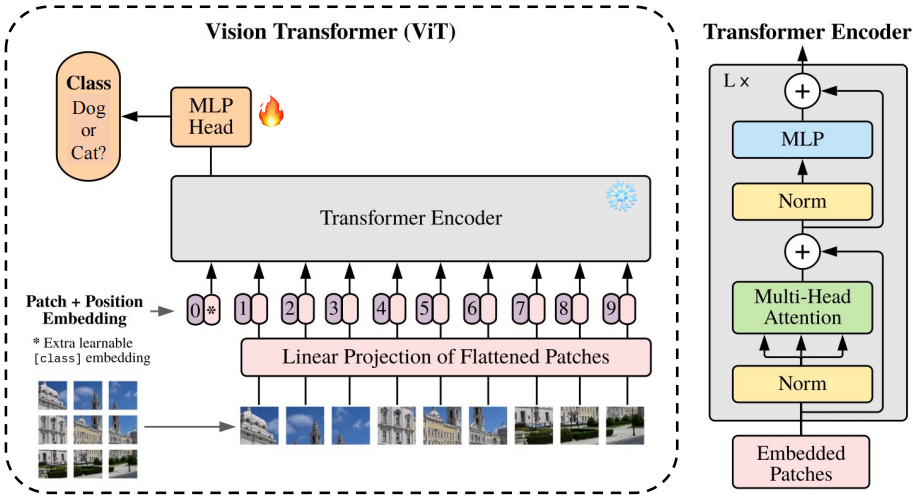
\includegraphics[width=0.78\linewidth]{figs/vit_overview.png}};
  \coordinate (xL)  at ($(img.north west)!0.19!(img.north east)$);
  \coordinate (xR)  at ($(img.north west)!0.74!(img.north east)$);
  \coordinate (yT)  at ($(img.north west)!0.345!(img.south west)$);
  \coordinate (yB)  at ($(img.north west)!0.545!(img.south west)$);
  \draw[red, dashed, thick] (xL |- yT) rectangle (xR |- yB);
  \node[red, anchor=north west, font=\scriptsize] at ($(img.south west)+(0,-0.12)$)
        {红色虚线框 = ImageEncoder 主体（12 层 Transformer Encoder，本人实现）};
\end{tikzpicture}
\caption{ViT-B/32 图像编码器的整体结构（图片来自课程模板）。
\textbf{红色虚线框}内的 12 层 Transformer Encoder 是 ImageEncoder 的主体，
也是本项目实现的部分；patch 嵌入、投影与 MLP 的细节见后续图。}
\label{fig:arch}
\end{figure}

% Experiment Objectives

\section{Objectives}

本项目要求在不训练的前提下，用纯 NumPy 复现 OpenCLIP ViT-B/32 图像编码器的前向计算。
输入是经过 CLIP 均值/方差归一化的 $[B,3,224,224]$ \texttt{float32} 图像，输出是对应的
$[B,512]$ 单位向量。模型权重课程已经给好（152 个张量，约 8785 万参数），
我只需要补全 starter 里 \texttt{image\_encoder.py} 的六处 \texttt{TODO}，
再用课程给的 \texttt{check.py} 分八个阶段和参考结果逐级比对。

我希望达到的目标是：
(1) 八个阶段全部 PASS，最大绝对误差在课程给定容差以内；
(2) 所有中间结果保持 \texttt{float32}，形状与参考一致；
(3) 代码能处理任意图像和任意 batch 大小，只依赖权重，不依赖参考数据；
(4) 按 README 能复现结果，代码放到 GitHub，报告正文控制在 5 页以内。

% Experiment Process
\section{Overview}
整个编码器就是一条前向的视觉 Transformer 管线（整体结构见图~\ref{fig:arch}），
数据流如图~\ref{fig:pipeline}。
$[B,3,224,224]$ 的图像按 $32\times32$ 切成 $7\times7=49$ 个 patch，展平成 $[B,49,3072]$；
再线性投影到 768 维，前面拼一个 CLS token，加上可学习位置编码，得到 $[B,50,768]$；
然后过 12 个 pre-LN Transformer block（每个 block 有注意力和 MLP 两条残差，
内部结构见图~\ref{fig:block}）；最后取 CLS 那一行，经过 \texttt{ln\_post} 和投影变成
$[B,512]$，再做 $L_2$ 单位化。

验证用的是课程给的 \texttt{check.py}。它每个阶段都读课程参考数组，用 \texttt{compare()}
逐元素比较：要求 \texttt{numpy} 数组、形状一致、\texttt{float32}、数值有限，再检查
\texttt{allclose}。容差方面 \texttt{preprocess} 是 $2\times10^{-6}$，
\texttt{output}/\texttt{batch} 是 $2\times10^{-5}$，其余阶段是 $2\times10^{-4}$。
\texttt{patches}/\texttt{tokens}/\texttt{block0}/\texttt{last\_tokens} 用前两张图，
\texttt{output} 用全部十张图，\texttt{batch} 用 $[1,0,1]$ 这种乱序且带重复的索引，
检查每行输出是否只取决于输入的图片。

我的运行环境是 Python 3.14.0、NumPy 2.2.6、Pillow 12.0.0、imageio 2.37.2，纯 CPU。
跑完八个阶段大约 90--120 秒，其中大部分时间花在 \texttt{assets} 阶段校验 326\,MB 权重
和十张图的 SHA-256 上。

% Figure

\begin{figure}[t]
\centering
\begin{tikzpicture}[font=\scriptsize,
  box/.style={draw, rounded corners=2pt, align=center, text width=3.15cm,
              minimum height=1.5cm, inner sep=2.5pt},
  given/.style={box, fill=gray!10, draw=gray!55},
  minebox/.style={box, fill=red!10, draw=red!70!black},
  ar/.style={-{Latex[length=1.8mm]}, thick}]
  \node[given] (in)  {输入图像\\$[B,3,224,224]$};
  \node[minebox, right=0.75cm of in]  (pat) {\mine{patchify}：切成 $7\times7$ 个 patch\\$[B,49,3072]$};
  \node[minebox, right=0.75cm of pat] (emb) {\mine{patch 投影} + \mine{CLS} + \mine{位置编码}\\$[B,50,768]$};
  \node[box, fill=red!4, draw=red!70!black, below=1.15cm of emb] (blk)
        {$\times 12$ Transformer Block（见图~\ref{fig:block}）\\$[B,50,768]$};
  \node[minebox, left=0.75cm of blk] (cls) {\mine{CLS 选择} + \mine{ln\_post} + 投影\\$[B,768]\to[B,512]$};
  \node[minebox, left=0.75cm of cls] (out) {\mine{$L_2$ 单位化}\\$[B,512]$};
  \draw[ar] (in)  -- (pat);
  \draw[ar] (pat) -- (emb);
  \draw[ar] (emb) -- (blk);
  \draw[ar] (blk) -- (cls);
  \draw[ar] (cls) -- (out);
  \node[font=\tiny, red!60!black, anchor=north west] at ($(out.south west)+(0,-0.25)$)
        {红框 = 本人实现（共 6 处）；灰框 = 课程给定};
  \node[font=\tiny, anchor=north west] at ($(out.south west)+(0,-0.62)$)
        {像素数不变：$3\times224\times224=49\times3072=150{,}528$};
\end{tikzpicture}
\caption{OpenCLIP ViT-B/32 的 ImageEncoder 前向数据流（箭头方向即数据流方向）。
红色标出的正是本人实现的六处：patchify、patch 投影、CLS 与位置编码、注意力与残差（Block 内部）、
CLS 选择 + \texttt{ln\_post} + 投影、$L_2$ 单位化；灰色是课程给出的预处理与参数加载。
CLIP 的文本塔不参与本项目。}
\label{fig:pipeline}
\end{figure}

\begin{figure}[t]
\centering
\begin{tikzpicture}[font=\scriptsize, node distance=0.5cm,
  b/.style={draw, rounded corners=2pt, align=center, minimum height=0.75cm,
            text width=1.7cm, inner sep=2pt},
  minebox/.style={b, fill=red!12, draw=red!70!black},
  given/.style={b, fill=gray!10, draw=gray!55},
  ar/.style={-{Latex[length=1.6mm]}, thick}]
  \node[given] (x) {$x$};
  \node[minebox,  right=of x]   (ln1) {LayerNorm};
  \node[minebox,  right=of ln1] (mha) {多头自注意力};
  \node[given, right=of mha] (a1)  {$\oplus$};
  \node[minebox,  right=of a1]  (ln2) {LayerNorm};
  \node[minebox,  right=of ln2] (mlp) {MLP + GELU};
  \node[given, right=of mlp] (a2)  {$\oplus$};
  \draw[ar] (x)   -- (ln1);
  \draw[ar] (ln1) -- (mha);
  \draw[ar] (mha) -- (a1);
  \draw[ar] (a1)  -- (ln2);
  \draw[ar] (ln2) -- (mlp);
  \draw[ar] (mlp) -- (a2);
  \draw[ar, red!70!black] (x.south)  -- ++(0,-0.5) -| (a1.south);
  \draw[ar, red!70!black] (a1.north) -- ++(0,0.5) -| (a2.north);
\end{tikzpicture}
\caption{单个 Transformer block（pre-LN，共 12 层）。红色是我实现的两条残差
$x+\mathrm{Attn}(\mathrm{LN}_1(x))$ 与 $u+\mathrm{MLP}(\mathrm{LN}_2(u))$ 以及注意力/MLP 内部；
灰色 $\oplus$ 是给定的逐元素相加。MLP 用精确 \texttt{erf}-GELU，线性层权重按 $[out,in]$ 存储。}
\label{fig:block}
\end{figure}

% Implementation Details
\section{Implementations}
需要我写的六处代码都在 \texttt{image\_encoder.py} 里，其余文件没有改动（红色为本人实现）。

\begin{enumerate}
  \item[(1)] \mine{\texttt{patchify}}：把 $[B,3,224,224]$ 切成 $7\times7$ 个 $32\times32$ 的 patch，
        展平成 $[B,49,3072]$。我先 \texttt{reshape}$(B,3,7,32,7,32)$，再
        \texttt{transpose}$(0,2,4,1,3,5)$，最后 \texttt{reshape}$(B,49,3072)$。
        行序是先行后列，必须和位置编码的 1--49 行一一对应。
  \item[(2)] \mine{\texttt{split\_heads}}：把 $[B,50,768]$ 拆成 $[B,12,50,64]$。
        \texttt{reshape}$(B,50,12,64)$ 把特征轴分成（head, head\_dim）两轴，
        再 \texttt{transpose}$(0,2,1,3)$ 把 head 轴移到 token 后面，让每个头独立做注意力。
  \item[(3)] \mine{缩放点积注意力}：$\mathrm{scores}=QK^\top/\sqrt{64}$，softmax 用给定的
        \texttt{attention\_weights}；$\mathrm{context}=AV$ 之后要先 \texttt{transpose}$(0,2,1,3)$
        再 \texttt{reshape} 合并头，最后过 \texttt{out\_proj}。缩放因子写成
        \texttt{np.float32(np.sqrt(...))}，原因见第~\ref{sec:debug}~节的 bug。
  \item[(4)] \mine{Transformer block}：两条残差 $r=x+\mathrm{Attn}(\mathrm{LN}_1(x))$、
        $u=\mathrm{LN}_2(r)$、\texttt{out}$=r+\mathrm{MLP}(u)$；MLP 是
        $\mathrm{GELU}(uW_1^\top+b_1)W_2^\top+b_2$。权重按 $[out,in]$ 存，所以统一乘 \texttt{.T}。
  \item[(5)] \mine{嵌入}：\texttt{patches} 乘 \texttt{patch\_weight}$^\top$（没有偏置），
        然后用 \texttt{concatenate} 把 CLS 拼到第 0 行，再加位置编码，得到 $[B,50,768]$。
  \item[(6)] \mine{\texttt{\_\_call\_\_}}：取 CLS 行 \texttt{tokens}$[:,0,:]$，过 \texttt{ln\_post}
        和投影（\texttt{visual.proj} 已经是 $[768,512]$，\textbf{不转置}），最后用给定的
        \texttt{unit\_vector} 做 $L_2$ 归一化。
\end{enumerate}

有两个容易搞错的约定：注意力和 MLP 的线性层权重按 $[out,in]$ 存（要乘 \texttt{.T}），
而输出投影 \texttt{visual.proj} 按 $[in,out]$ 存（不转置）；这个模型没有 LayerScale，
每个 block 只有上面那两条残差。接口保持和 \texttt{helpers.py} 一致，没有改课程任何给定文件。

\paragraph{形状变化.} 六处里形状变化最绕的是 \texttt{split\_heads}，我拿它来说：
输入 $[B,50,768]$ 里，每个 token 的 768 维其实是 12 个头各 64 维拼起来的。
\texttt{reshape}$(B,50,12,64)$ 只改变视图、不动数据顺序，把最后一维拆成 $(12,64)$；
但内存里头的位置仍然排在 token 维度后面，所以还要 \texttt{transpose}$(0,2,1,3)$
把 12 移到第 2 轴，得到 $[B,12,50,64]$，此时每个头是一个独立的 $[50,64]$ 矩阵，
可以直接算 $QK^\top$。算完 $AV$ 得到 $[B,12,50,64]$，合并时必须先
\texttt{transpose}$(0,2,1,3)$ 回到 $[B,50,12,64]$ 再 \texttt{reshape} 成 $[B,50,768]$；
如果直接 \texttt{reshape}，特征会按头交错拼接，和参考对不上。

\section{Results}

八个阶段全部 PASS（官方 \texttt{check.py}，本机实测），各阶段误差见表~\ref{tab:err}。

\begin{table}[H]
\centering
\caption{各阶段数值误差（\texttt{check.py --stage all} 实测；容差为 \texttt{atol}/\texttt{rtol}）}
\label{tab:err}
\small
\begin{tabular}{llrrr}
\toprule
阶段 & 输出形状 & max abs & mean abs & 容差 \\
\midrule
\texttt{assets}      & 152 张量 / 10 组图 & --- & --- & SHA-256 \\
\texttt{preprocess}  & $(10,3,224,224)$   & $0.000\times10^{0}$ & $0.000\times10^{0}$ & $2\times10^{-6}$ \\
\texttt{patches}     & $(2,49,3072)$      & $0.000\times10^{0}$ & $0.000\times10^{0}$ & $2\times10^{-4}$ \\
\texttt{tokens}      & $(2,50,768)$       & $7.153\times10^{-6}$ & $2.597\times10^{-7}$ & $2\times10^{-4}$ \\
\texttt{block0}      & $(2,50,768)$       & $7.540\times10^{-6}$ & $2.455\times10^{-7}$ & $2\times10^{-4}$ \\
\texttt{last\_tokens}& $(2,50,768)$       & $4.196\times10^{-5}$ & $2.438\times10^{-6}$ & $2\times10^{-4}$ \\
\texttt{output}      & $(10,512)$         & $7.302\times10^{-7}$ & $8.244\times10^{-8}$ & $2\times10^{-5}$ \\
\texttt{batch}       & $(3,512)$          & $4.992\times10^{-7}$ & $7.769\times10^{-8}$ & $2\times10^{-5}$ \\
\bottomrule
\end{tabular}
\end{table}

官方检查输出（节选，八行均为 PASS）：

{\footnotesize
\begin{verbatim}
assets       PASS: 152 matching visual tensors and ten image/reference pairs
preprocess   PASS shape=(10, 3, 224, 224) max_abs=0.000e+00 mean_abs=0.000e+00
patches      PASS shape=(2, 49, 3072) max_abs=0.000e+00 mean_abs=0.000e+00
tokens       PASS shape=(2, 50, 768) max_abs=7.153e-06 mean_abs=2.597e-07
block0       PASS shape=(2, 50, 768) max_abs=7.540e-06 mean_abs=2.455e-07
last_tokens  PASS shape=(2, 50, 768) max_abs=4.196e-05 mean_abs=2.438e-06
output       PASS shape=(10, 512) max_abs=7.302e-07 mean_abs=8.244e-08
batch        PASS shape=(3, 512) max_abs=4.992e-07 mean_abs=7.769e-08
Requested numerical checks passed. The reference file is never an encoder input.
\end{verbatim}
}

另外我用 \texttt{run.py} 对 10 张图导出 \texttt{output\_tokens.npz}，输出
\texttt{Saved (10, 512)}，形状、\texttt{float32}、有限性校验都通过。

误差方面，\texttt{preprocess}/\texttt{patches} 为 0，因为预处理逐位一致、patchify 只是挪内存；
从 \texttt{tokens} 开始出现 $10^{-6}$ 量级误差，来自 \texttt{float32} 矩阵乘的累加顺序
（和 BLAS 实现有关）以及 \texttt{erf}-GELU 的逐元素舍入；12 层累积后 \texttt{last\_tokens}
到 $4.2\times10^{-5}$，仍在内部容差 $2\times10^{-4}$ 以内；最后只取 CLS 一行再做 $L_2$ 归一化，
绝对误差反而降到 $7.3\times10^{-7}$。这些差异都来自浮点运算顺序和数学库实现，不是算法不同。

\section{Discussion}

\paragraph{\mine{一个修复的 bug：float32 被静默提升为 float64.}}\label{sec:debug}
写完注意力分数后我跑 \texttt{check.py --stage block0}，报错
\texttt{block0 FAIL: block0: use float32}。这是 \texttt{check.py} 对 \texttt{dtype} 的硬性检查，
说明数值可能对、但返回的数组类型不对。打印后确认 \texttt{scores.dtype} 是 \texttt{float64}，
问题出在缩放那一行：

\[\texttt{scores = q @ np.swapaxes(k,-1,-2) / np.sqrt(self.head\_dim)}\]

\texttt{self.head\_dim} 是 Python 的 \texttt{int}，\texttt{np.sqrt(64)} 返回 \texttt{np.float64}
标量，\texttt{float32} 数组除以它会被类型提升规则悄悄变成 \texttt{float64}，后面所有张量都被污染。
我把缩放因子改成 \texttt{scale = np.float32(np.sqrt(self.head\_dim))}，\texttt{block0} 立刻 PASS
（max abs $7.5\times10^{-6}$）。可见数值逻辑本来就是对的，只是 dtype 约定被破坏；
全程 \texttt{float32} 还能省一半内存和计算。

\paragraph{贡献与所用帮助.}
六个 \texttt{TODO} 都是我自己写的，环境搭建、README 和这份报告的整理也是我做的。
外部帮助主要有：课程提供的 starter 代码和注释、\texttt{helpers.py}、\texttt{check.py} 的容差说明、
课程 PPT（slide 39--70，对应 \texttt{PPT-CODE-MAP.txt}）；另外我用 AI 助手帮忙排查环境问题
（例如 anaconda 解释器里 conda 版 Pillow 会让 \texttt{preprocess} 出现
$4.1\times10^{-1}$ 的假失败，换成系统 Python 3.14 后就逐位一致）、核对维度和权重布局，
以及润色文字。代码逻辑和数值结论我都自己验证过。

\paragraph{小结.} 这个项目里真正写循环和乘法的时间不多，大部分时间花在把形状、
权重布局、CLS 位置这些约定对齐上；八个阶段全 \texttt{PASS}，
说明纯 NumPy 的实现和课程参考在数值上是等价的。

\paragraph{代码与复现.} 代码放在 GitHub，仓库地址：

\noindent\texttt{https://github.com/yyxbhsj/szu-python-project1-vit-b32}

\noindent 仓库里有 \texttt{image\_encoder.py}、\texttt{README.md}（环境、命令和预期输出）
以及本报告的 \LaTeX{} 源码和 PDF。复现时把仓库里的 \texttt{image\_encoder.py} 覆盖课程 starter
中的同名文件，装好 \texttt{requirements.txt} 后运行 \texttt{python check.py --stage all} 即可。

\newpage

% ============================================================
% 批阅与成绩评定页
% ============================================================

% 绘制正文外框（包含批阅区域）
\begin{tikzpicture}[remember picture, overlay]
  \draw[thick]
    ($(current page.north west)+(2cm,-3cm)$)
    rectangle
    ($(current page.south east)+(-2cm,3.5cm)$);
\end{tikzpicture}

\vspace{1cm}

% 批阅区
\noindent \textbf{指导教师批阅意见：}
\vspace{6cm}
\hfill

\vspace{1cm}

\noindent \textbf{成绩评定：}
\vspace{2cm}
\hfill

\vspace{1cm}

\noindent
\hfill
\textbf{指导教师签字：}\quad\quad\quad\quad\quad\\[0.5cm]

\hfill
\textbf{年}\quad\quad
\textbf{月}\quad\quad
\textbf{日}\quad

\vspace{1cm}

% 备注部分
\noindent \textbf{备注：}

% 框外的注释
\begin{tikzpicture}[remember picture, overlay]
  \node[
    anchor=north west,
    inner sep=0pt,
    text width=\dimexpr\paperwidth-4cm\relax
  ] at ($(current page.south west)+(2cm,3.1cm)$) {
    \begin{minipage}{\dimexpr\paperwidth-4cm\relax}
      \small
      \noindent
      \textbf{注：}\;1、报告内的项目或内容设置，可根据实际情况加以调整和补充。\\[0.2cm]
      \phantom{\textbf{注：}\;}2、教师批改学生实验报告时间应在学生提交实验报告时间后 10 日内。
    \end{minipage}
  };
\end{tikzpicture}

% ============================================================
%                      文档结束
% ============================================================

\end{document}
